\documentclass[10pt]{article}
\usepackage[T1]{fontenc}
\usepackage[utf8]{inputenc}
\usepackage{lmodern,amsmath,amssymb,amsthm,graphicx,booktabs,microtype}
\usepackage[top=.72in,bottom=.72in,left=1in,right=1in]{geometry}
\usepackage{xcolor,titlesec,enumitem,xurl,hyperref,placeins}
\definecolor{ink}{HTML}{202C30}
\definecolor{accent}{HTML}{285A52}
\definecolor{rulecolor}{HTML}{D9E0DA}
\color{ink}
\hypersetup{pdftitle={Certified Block Overlap in Subset Sum},
  pdfauthor={Jonathan R. Landers},hidelinks}
\titleformat{\section}{\normalfont\sffamily\large\bfseries\color{accent}}{\thesection}{.65em}{}
\titlespacing*{\section}{0pt}{10pt plus 2pt}{5pt}
\setlength{\parindent}{0pt}
\setlength{\parskip}{3pt plus .5pt}
\setlength{\emergencystretch}{2em}
\setlength{\abovedisplayskip}{6pt plus 1pt}
\setlength{\belowdisplayskip}{6pt plus 1pt}
\setlength{\textfloatsep}{11pt plus 2pt minus 2pt}
\setlist[enumerate]{leftmargin=*,itemsep=1pt,topsep=3pt}
\raggedbottom
\newtheorem{theorem}{Theorem}
\newtheorem{lemma}[theorem]{Lemma}
\newtheorem{corollary}[theorem]{Corollary}
\newtheorem{proposition}[theorem]{Proposition}
\newcommand{\poly}{\operatorname{poly}}
\newcommand{\supp}{\mathcal S}
% Generated from hash-checked validation.json; do not hand edit.
\newcommand{\ExhaustiveInputs}{462}
\newcommand{\PartitionChecks}{1,386}
\newcommand{\RandomInputs}{120}
\newcommand{\TargetChecks}{37,055}
\newcommand{\LargeItems}{300}
\newcommand{\LargeBlocks}{100}
\newcommand{\LargeIntervals}{897}
\newcommand{\LargeCandidates}{7,966}
\newcommand{\LargeYesNodes}{101}
\newcommand{\LargeNoNodes}{1}


\begin{document}
{\LARGE\sffamily\bfseries Certified Block Overlap in Subset Sum}\par
\vspace{3pt}
{\large\sffamily Small local dictionaries, bounded search, paid discovery}\par
\vspace{5pt}
{\small Jonathan R. Landers \hfill November 2026}\par
\textcolor{rulecolor}{\rule{\linewidth}{.6pt}}

\textbf{Abstract.}
With $n$ input weights, subset sum can admit a short exact search even when
all $2^n$ sums are distinct. We divide sorted positive weights into small blocks and list each
block's distinct sums. An interval test bounds the choices that survive in
each block; their product bounds the search tree. A dynamic program minimizes
this product over contiguous partitions with at most $b$ items per block.
Writing the optimum as $K_b$ and binary input length as $L$, finding the
partition and solving the instance take $\poly(L)(2^b+K_b)$ bit operations,
where $\poly(L)$ is a polynomial factor in $L$.
We prove the bound, give a robust family with $K_3=1$, and verify the
implementation exhaustively on small inputs.

\section{Why local separation helps}
Subset sum asks whether some selection of positive integer weights totals a
specified integer target. Merging repeated sums is one shortcut.
We study another: \emph{separation} between local sums can rule out most
choices, even when all global sums differ.

Consider the blocks $(2,3,4)$ and $(20,30,40)$. The lower block totals $9$.
To reach $37$, the higher block must contribute between $28$ and $37$.
Only $30$ fits, leaving $7$, which the lower block can reach.
For target $38$, the same choice leaves $8$, which it cannot reach.
The interval test rules out whole groups, but a surviving choice still
needs an exact check. We bound this search for every target and include
the cost of finding the partition.

The meet-in-the-middle algorithm of Horowitz and Sahni~\cite{hs}
uses $O^*(2^{n/2})$ time; Schroeppel and Shamir~\cite{ss} retain that time
with $O^*(2^{n/4})$ space. Here $O^*$ suppresses factors polynomial in
encoded input length. Ordered-sum constructions~\cite{ordered} already show
that distinct sums can coexist with efficient decision.
Li and Ye~\cite{partial} improve on the classical $1/2$ exponent using
compatibility tests on partial representations. We instead seek an
easily checked condition that makes a particular input easy.

Let $a=(a_1,\ldots,a_n)\in\mathbb Z_{>0}^n$, $t\in\mathbb Z$, and
$[n]=\{1,\ldots,n\}$. The required output is an index set $U\subseteq[n]$
such that $\sum_{i\in U}a_i=t$, or a correct NO answer. Such a set $U$ is a
\emph{witness}.
Equal values remain distinct indexed items; the empty selection is allowed.
Let $L$ be the binary encoding length of $(a,t)$, including delimiters.
Then $n=O(L)$, and sums and witness masks (one bit per original item)
have $O(L)$ bits. All logarithms are base two.
The notation $\poly(L)$ hides a uniform polynomial, with no extra
exponential parameter. Numeric magnitude is different: for $t\ge0$, Bringmann's randomized
$\widetilde O(n+t)$ algorithm~\cite{pseudo} is near-linear
pseudopolynomial time, not polynomial time in the binary length of $t$.
The tilde suppresses logarithmic factors.

\section{Local sums and the interval test}
Sort the items as $w_1\le\cdots\le w_n$, breaking ties by original index and
retaining that index map. Choose an integer block-size limit $1\le b\le n$.
Partition the indices into $m$ nonempty blocks using integer cuts
$0=v_0<v_1<\cdots<v_m=n$, with $v_j-v_{j-1}\le b$.
The $j$th block is $B_j=\{v_{j-1}+1,\ldots,v_j\}$.
Define its distinct-sum set $S_j$ and the total weight $P_j$ of all lower blocks:
\begin{equation}\label{eq:local}
 S_j=\left\{\sum_{i\in U}w_i:U\subseteq B_j\right\},
 \qquad P_j=\sum_{i=1}^{v_{j-1}}w_i.
\end{equation}
Store the sorted distinct values in $S_j$, keeping one original-index witness
per value. If higher blocks leave residual target $r$, a completion using
$s\in S_j$ needs a lower contribution $r-s\in[0,P_j]$.

A set of attainable sums is also called a \emph{support}. Bringmann,
Fischer, and Nakos~\cite{support} compute the support $\mathcal S_{\le t}$
of all attainable sums up to a nonnegative target $t$ in randomized time
$\widetilde O(|\mathcal S_{\le t}|\sqrt n)$. We build only small local
supports, avoiding the full set in the family below.

\begin{lemma}[Sound exclusion and merging]\label{lem:exact}
Only sums $s\in S_j\cap[r-P_j,r]$ can occur in a completion.
Keeping one witness per distinct block sum preserves existence and recovery
of one full witness.
\end{lemma}
\begin{proof}
Every lower selection has sum $u$ with $0\le u\le P_j$; $s+u=r$ implies
$r-P_j\le s\le r$. Conversely, two selections within $B_j$ with equal sum
leave the same residual and the same unprocessed blocks. Substituting one
for the other preserves a solution and cannot reuse an index, because
blocks are disjoint.
\end{proof}

The interval $[s,s+P_j]$ contains every residual target that could use local
sum $s$. Write $\mathcal B=(B_1,\ldots,B_m)$ for the partition.
Its maximum local overlaps $\kappa_j$ and their product $K(\mathcal B)$ are
\begin{equation}\label{eq:overlap}
 \kappa_j=\max_{z\in\mathbb Z}|S_j\cap[z-P_j,z]|,
 \qquad K(\mathcal B)=\prod_{j=1}^m\kappa_j,
 \qquad 1\le\kappa_j\le |S_j|\le2^b .
\end{equation}
When the partition is fixed, we abbreviate $K(\mathcal B)$ as $K$.
Intervals are closed: sums exactly $P_j$ apart can both qualify.
Figure~\ref{fig:intervals} makes this endpoint issue visible.

\begin{figure}[htbp]
\centering
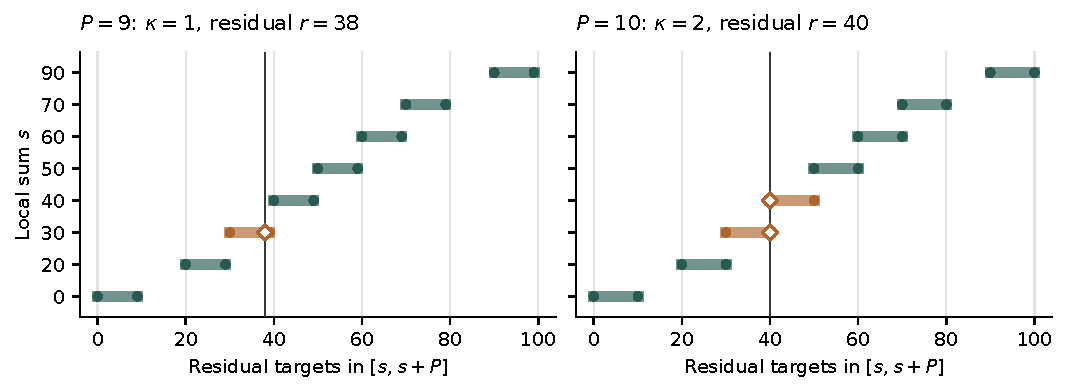
\includegraphics[width=.97\linewidth]{block_overlap_geometry.pdf}
\caption{\textbf{Overlap is a branching certificate.}
Segments show $[s,s+P]$ for the local sums of $(20,30,40)$;
$P$ and $\kappa$ denote this block's lower total and maximum overlap.
Orange marks the choices that contain the indicated residual.
For $P=9$, at most one choice survives. For $P=10$, residual $40$
lies at the shared endpoints for $s=30$ and $s=40$, so $\kappa=2$.
The original example uses $P=9$; the right panel varies the lower total.}
\label{fig:intervals}
\end{figure}

\section{Bounding the search tree}
Search blocks in descending order; depth counts processed blocks, starting at zero.
At block $j$, use two binary searches
to locate $S_j\cap[r-P_j,r]$, then recurse on each qualifying sum $s$
with residual $r-s$. At depth $m$, accept precisely residual zero.
Reject $t\notin[0,\sum_iw_i]$ immediately.

\begin{theorem}[Fixed-partition search]\label{thm:search}
The algorithm is exact. Let $N(\mathcal B,t)$ count the nodes in its
complete search tree for target $t$. Then
\begin{equation}\label{eq:tree}
 N(\mathcal B,t)\le
 1+\sum_{\ell=1}^m\prod_{h=m-\ell+1}^m\kappa_h
 \le(m+1)K(\mathcal B).
\end{equation}
There are at most $K(\mathcal B)$ complete paths, each choosing one sum per block.
After construction of the
local dictionaries, its bit cost is at most $\poly(L)K(\mathcal B)$.
An early YES may stop sooner.
\end{theorem}
\begin{proof}
Induct on the number of remaining blocks. With no blocks, precisely residual
zero is attainable. Lemma~\ref{lem:exact} discards no solution and justifies
the stored representative for every surviving local sum. Applying the
induction hypothesis to these children proves both YES and NO correctness.

At depth $\ell$, each preceding node has at most $\kappa_{m-\ell+1}$
children, independently of its residual. Multiplying these deterministic
upper bounds and summing levels gives the first inequality in
\eqref{eq:tree}. Since every $\kappa_h\ge1$, every partial product is at
most $K(\mathcal B)$, proving the second. Binary searches take
$O(\log(|S_j|+1))=O(b+1)$ comparisons per internal node.
Charge each generated child once; sums, residuals, and masks have $O(L)$
bits. Witness assembly and its final weighted-sum check are polynomial.
All these charges fit the stated bit bound.
\end{proof}

The bound includes failed branches and NO instances; it uses no independence
assumption. Merging equal-sum witnesses preserves existence, not solution counts.

\section{Finding and building the partition}
A small product helps only if its partition is cheap to find.
For a contiguous block, the lower total depends only on its starting
position. It stays fixed as earlier cuts change, giving a dynamic program.

Let $H_v=\sum_{i=1}^vw_i$, with $H_0=0$, be the prefix totals.
For $1\le u\le v\le n$ and
$v-u+1\le b$, let $S_{u,v}$ be the distinct sums of $w_u,\ldots,w_v$ and
define $\kappa(u,v)=\max_{z\in\mathbb Z}|S_{u,v}\cap[z-H_{u-1},z]|$.
Let $D(v)$ be the minimum overlap product over permitted partitions of the first $v$ items.
The exact integer recurrence
\begin{equation}\label{eq:dp}
 D(0)=1,\qquad
 D(v)=\min_{\max(1,v-b+1)\le u\le v}
          D(u-1)\kappa(u,v),\qquad K_b=D(n)
\end{equation}
stores a minimizing predecessor for each $v$.

\begin{theorem}[Optimal contiguous discovery and total cost]\label{thm:paid}
The recurrence finds
$K_b=\min_{\mathcal B}K(\mathcal B)$ over all contiguous sorted partitions
whose blocks contain at most $b$ items.
For the returned partition of $m$ blocks, let $T(a,t;b)$ be the total bit-operation count and
$\mathrm{Space}(a,t;b)$ the peak workspace in bits.
Including sorting, construction, optimization, reconstruction, and search,
\begin{equation}\label{eq:paid}
 \boxed{\quad T(a,t;b)\le\poly(L)(2^b+K_b),\qquad
             \mathrm{Space}(a,t;b)\le\poly(L)2^b.\quad}
\end{equation}
Optimality refers to this partition family and product bound.
\end{theorem}
\begin{proof}
Every partition of the first $v$ items has a last block $[u,v]$.
Its final factor $\kappa(u,v)$ uses $H_{u-1}$, regardless of earlier cuts.
Replacing the preceding partition by an optimum cannot increase the
product. Induction proves \eqref{eq:dp} and predecessor reconstruction.

There are at most $nb$ candidate blocks. For a block of length $\ell$,
start with $(0,\varnothing)$ and repeatedly merge the current sorted
sum list with its translate by the next weight, coalescing equal sums
and retaining a witness. List sizes are at most $2^h$ after $h$ items;
the total merge work is $O(\sum_{h=1}^{\ell}2^h)=O(2^\ell)$
arithmetic/comparison operations.

List a candidate support as $s_1<\cdots<s_q$, with $q=|S_{u,v}|$.
A sliding window moves its left
endpoint forward until $s_{\rm right}-s_{\rm left}\le H_{u-1}$,
where \emph{left} and \emph{right} index the window endpoints.
The largest window equals $\kappa(u,v)$: any nonempty eligible interval
can move its right endpoint to its largest contained support value
without losing a contained value. Each endpoint moves at most $q$ times,
so scoring takes $O(q)$ comparisons.

Thus discovery costs $O(n\log(n+1)+nb2^b)$ operations.
Discard a candidate list after scoring, store its score, and rebuild only
the chosen block lists, adding $O(n2^b)$ operations. Each DP candidate
product is at most $2^v$, so it uses at most $n+1$ bits.
All other represented integers and witnesses also have polynomial bit length.
Theorem~\ref{thm:search} then gives \eqref{eq:paid}.
More explicitly, schoolbook integer arithmetic permits the conservative bound
\[
 O\!\left(L^2\left[n\log(n+1)+nb2^b+(m+1)(b+1)K_b\right]\right).
\]

Store $O(nb)$ scores, predecessors, one temporary candidate list, and the
chosen lists, which have at most $m2^b$ records. Depth-first search keeps
one path and pending siblings: at most $1+m(2^b-1)$ pending nodes.
Each record uses polynomially many bits, proving the space bound.
\end{proof}

\textbf{Reference algorithm.}
\begin{enumerate}
\item Sort with original indices; compute prefix totals $H_v$.
\item Construct and score every candidate block of length at most $b$.
\item Evaluate \eqref{eq:dp} using exact integer products; reconstruct its cuts
and rebuild their witnessed dictionaries.
\item Search downward using Lemma~\ref{lem:exact}; verify any recovered witness
against the original input. Exhausting every surviving branch certifies NO.
\end{enumerate}
For $n=0$, take the empty partition and $K_b=1$: only $t=0$ is reachable.

\begin{corollary}[An efficiently recognizable tractable class]\label{cor:poly}
Fix integers $c\ge1$ and $d\ge0$. For nonempty inputs choose
$b=\min\{n,\max\{1,\lfloor c\log_2(L+1)\rfloor\}\}$.
The class $K_b\le(L+1)^d$ is recognizable and solvable in polynomial
bit time, without a supplied partition.
\end{corollary}
\begin{proof}
Discovery is polynomial because $2^b$ is polynomial in $L$;
$\lfloor c\log_2(L+1)\rfloor$ is computable as the bit length of
$(L+1)^c$ minus one.
Compare the computed integer $K_b$ with the threshold and apply
Theorem~\ref{thm:paid} on accepted inputs.
\end{proof}

Other algorithms exploit different structure. Bringmann and
Wellnitz~\cite{dense} study dense inputs, with algorithms and conditional
lower bounds. For a nonempty integer set $A$, its \emph{sumset} is
$A+A=\{x+y:x,y\in A\}$.
Randolph and W\k{e}grzycki~\cite{doubling} use its additive doubling $|A+A|/|A|$.
Our $\kappa_j$ instead counts local choices compatible with a lower total.

Increasing $b$ cannot increase $K_b$: every earlier partition remains
available. But larger blocks can cost more to build. At $b=n$, a single
block gives $K_b=1$, yet its support may contain $2^n$ records.
This is why the bound charges $2^b$ separately.
Stored dictionaries and generated sums also drive time--space methods
such as OpenAI's low-space preprint~\cite{space}, which uses a different
randomized construction and word model.

\section{Many distinct sums, one search path}
For an integer $m\ge1$, take $m$ sorted triples. For $j=0,\ldots,m-1$,
assign the following weights to block $B_{j+1}$:
\begin{equation}\label{eq:family}
 \{w_i:i\in B_{j+1}\}=10^j\{2,3,4\},\quad n=3m,
 \qquad
 S_{j+1}=10^j\{0,2,3,4,5,6,7,9\}.
\end{equation}
Multiplication by $10^j$ scales each element of the displayed sets.
The total below block $j+1$ is
$P_{j+1}=9\sum_{h=0}^{j-1}10^h=10^j-1$.
Every gap between its consecutive support values is at least $10^j$,
strictly exceeding $P_{j+1}$. Hence every $\kappa_j=1$ and $K_3=1$.
The search visits at most $m+1$ nodes for any target.

Each triple's eight selections produce eight different decimal digits,
and no digit carries into the next block. The $8^m=2^n$ global sums are
therefore all distinct. Only $8m$ local records are retained for the
triple partition. Because $b=3$, discovery is polynomial, too:
the algorithm never builds the global support.

A sequence is \emph{superincreasing} if each weight exceeds the sum of
all earlier weights. This family fails that condition: $4\cdot10^j<
2\cdot10^j+3\cdot10^j$. The maximum-core greedy scan used in the
core-and-exceptions approach~\cite{core} keeps the first two items of each
triple and rejects the third. Indeed, before each triple its retained total
is $5(10^j-1)/9<10^j$; the first two items exceed the preceding retained
total, while the third does not. That route leaves $m$ exceptions and its
enumeration bound is exponential. This compares sufficient bounds, not
lower bounds against other algorithms.

\begin{proposition}[Irregular scales and perturbations]\label{prop:robust}
For blocks $j=1,\ldots,m$, replace the weights in $B_j$ by
$\{2M_j+e_{j,2},3M_j+e_{j,3},4M_j+e_{j,4}\}$, where
$M_j,E_j\in\mathbb Z_{\ge0}$ are a scale and an error bound.
The integer errors $e_{j,h}$ satisfy $|e_{j,h}|\le E_j$ for
$h\in\{2,3,4\}$; $P_j$ is the actual total of preceding triples. If
\begin{equation}\label{eq:robust}
 M_j-3E_j>P_j\qquad\text{for every }j,
\end{equation}
the triples form a contiguous sorted partition with $\kappa_j=1$,
all $2^{3m}$ global sums are distinct, and $b=3$ gives polynomial bit time.
\end{proposition}
\begin{proof}
An unperturbed difference between two distinct local subset sums has
absolute value at least $M_j$. Each of the three errors appears in their
difference with coefficient in $\{-1,0,1\}$, changing it by at most $3E_j$.
Thus every local difference remains larger than $P_j$.
Condition \eqref{eq:robust} also ensures positive weights, increasing order
within each triple, and a new smallest weight exceeding the earlier total.
The triples are therefore permitted sorted blocks with unit overlap.
For two different global selections, their highest differing block contributes
a difference larger than the total of all lower blocks; cancellation is
impossible. Apply Theorem~\ref{thm:paid}.
\end{proof}

\begin{figure}[tbp]
\centering
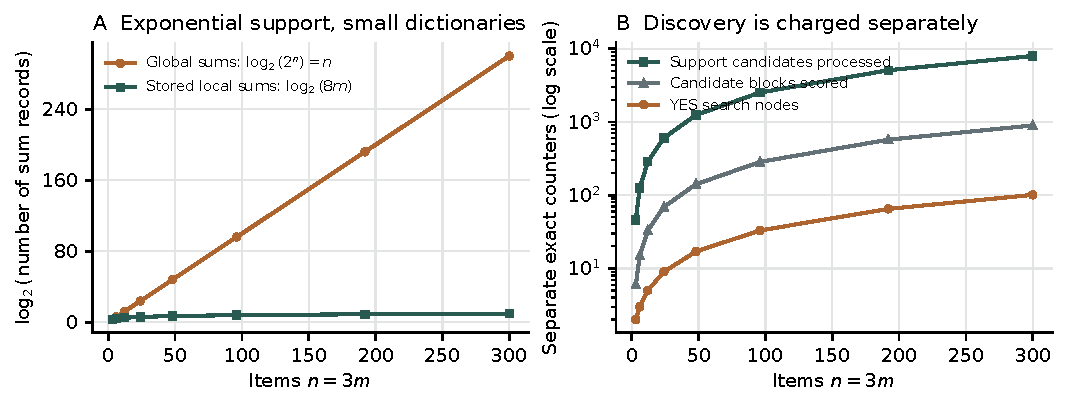
\includegraphics[width=.97\linewidth]{block_overlap_scaling.pdf}
\caption{\textbf{The separated family, with discovery visible.}
With $b=3$ and $m\in\{1,2,4,8,16,32,64,100\}$, panel A compares global
and stored local support sizes on a base-two logarithmic scale.
Panel B separates construction counters from search nodes for the
all-$7$ YES target. Support candidates include discovery and rebuilding.
These counters are neither timings nor uniform bit operations; they
are not added together.}
\label{fig:scaling}
\end{figure}

\FloatBarrier
\section{Verification and scope}
The standard-library solver uses exact integers and returns original indices.
An independent checker enumerates subsets and all admissible cut sets on
small inputs. The saved record reports:
\begin{center}
\begin{tabular}{lr}
\toprule
Check or constructed-example counter & Count\\
\midrule
All sorted multisets of $0$--$6$ items from $\{1,\ldots,5\}$ & \ExhaustiveInputs\\
Partition-optimality checks, $b\in\{1,2,3\}$ & \PartitionChecks\\
Additional seeded random inputs, at most $12$ items & \RandomInputs\\
Decision/witness comparisons against exhaustive subsets & \TargetChecks\\
\midrule
Candidate blocks scored, $n=\LargeItems$, $b=3$ & \LargeIntervals\\
Support candidates, including reconstruction & \LargeCandidates\\
Search nodes: all-$7$ YES target / leading-$8$ NO target & \LargeYesNodes{} / \LargeNoNodes\\
\bottomrule
\end{tabular}
\end{center}
Each tested target checks the decision, the original-index witness when
present, and \eqref{eq:tree}'s $(m+1)K$ envelope.
Boundary checks cover closed endpoints, duplicate weights, empty inputs,
and invalid weights. The seed for the random inputs is $20261104$.
For the \LargeItems-item example, the NO target is
$8\cdot10^{\LargeBlocks-1}$; the global count $2^{\LargeItems}$ follows
from the proof, not exhaustive enumeration. Global support distinctness is
also checked directly on the first one, two, and three triples.
These are correctness checks, not timing benchmarks.

The source directory contains \texttt{solver.py}, \texttt{verify.py},
and \texttt{validation.json}, which records their SHA-256 hashes.
From the repository root, run
\texttt{python} \path{notes/01-certified-coverage/block-overlap/verify.py} to
repeat the checks, or run the same directory's \texttt{build\_note.py} to
rebuild the paper. The builder checks hashes and citations, regenerates
plots and numerical macros, records \texttt{paper\_evidence.json}, and
enforces six pages. It preserves the original verification record.

\textbf{Relation to distribution shaping.}
For a fixed partition, $\log_2K=\sum_{j=1}^m\log_2\kappa_j$.
This sum could motivate a statistical model across random inputs,
but does not itself imply a lognormal law. That requires assumptions on
the input distribution and the terms' dependence.
Changing an axis leaves the computation unchanged; the saving comes
from bounded overlap.

\textbf{Prior work and limits.}
Singleton blocks $B_j=\{j\}$ with $w_j>P_j$ recover the classical superincreasing
case. Earlier ordered-sum constructions already combine distinct
subset sums with efficient knapsack decision~\cite{ordered}; that report's
abstract establishes precedent, not equivalence with this overlap bound.
We give a costed proof and checked implementation.
Novelty assessment, comparative timings, and partitions beyond contiguous
sorted blocks remain open. Small $2^b+K_b$ guarantees an efficient route;
large $K_b$ does not prove hardness.

\begin{thebibliography}{10}
\small
\setlength{\itemsep}{2pt}
\setlength{\parskip}{0pt}
\bibitem{hs} E. Horowitz and S. Sahni.
\emph{Computing Partitions with Applications to the Knapsack Problem}.
Journal of the ACM 21(2), 277--292, 1974.
\href{https://doi.org/10.1145/321812.321823}{doi:10.1145/321812.321823}.
\bibitem{ss} R. Schroeppel and A. Shamir.
\emph{A $T=O(2^{n/2})$, $S=O(2^{n/4})$ Algorithm for Certain NP-Complete Problems}.
SIAM Journal on Computing 10(3), 456--464, 1981.
\href{https://doi.org/10.1137/0210033}{doi:10.1137/0210033}.
\bibitem{ordered} M. D. Atkinson, A. Negro, and N. Santoro.
\emph{Sums of Lexicographically Ordered Sets}.
Carleton University Technical Report TR-100, May 1987.
\href{https://carleton.ca/scs/research/scs-technical-reports/technical-reports-1987/tr-100-sums-of-lexicographically-ordered-sets/}{Institutional abstract}.
\bibitem{partial} B. Li and L. Ye.
\emph{Subset Sum via Partial Match}.
Preprint, version 2, November 2, 2026.
\href{https://arxiv.org/abs/2610.10446v2}{arXiv:2610.10446v2}.
\bibitem{pseudo} K. Bringmann.
\emph{A Near-Linear Pseudopolynomial Time Algorithm for Subset Sum}.
SODA, 2017.
\href{https://arxiv.org/abs/1610.04712v2}{arXiv:1610.04712v2}.
\bibitem{support} K. Bringmann, N. Fischer, and V. Nakos.
\emph{Beating Bellman's Algorithm for Subset Sum}.
SODA, 2025.
\href{https://arxiv.org/abs/2410.21942v1}{arXiv:2410.21942v1}.
\bibitem{dense} K. Bringmann and P. Wellnitz.
\emph{On Near-Linear-Time Algorithms for Dense Subset Sum}.
SODA, 2021.
\href{https://arxiv.org/abs/2010.09096}{arXiv:2010.09096}.
\bibitem{doubling} T. Randolph and K. W\k{e}grzycki.
\emph{Parameterized Algorithms on Integer Sets with Small Doubling:
Integer Programming, Subset Sum and $k$-SUM}.
ESA, 96:1--96:19, 2024.
\href{https://doi.org/10.4230/LIPIcs.ESA.2024.96}{doi:10.4230/LIPIcs.ESA.2024.96}.
\bibitem{space} OpenAI.
\emph{A Low-Space Algorithm for Worst-Case Subset Sum}.
Preprint dated September 26, 2026;
\href{https://github.com/openai/math/blob/7ef5c0cc5ca4b0e072b7a050fca09ab24bc6fa3a/preprints/A-Low-Space-Algorithm-for-Worst-Case-Subset-Sum-September-26-2026/paper.pdf}{fixed repository version}.
\bibitem{core} J. R. Landers.
\emph{How Far from Easy? Structural Distance in Subset Sum}.
Working draft, 2026. Repository Note V,
\href{https://github.com/jonland82/exponential-search-spaces/tree/master/notes/05-structural-distance}{source and evidence}.
\end{thebibliography}
\end{document}
